% !TEX encoding = UTF-8
% !TEX TS-program = pdflatex
% !TEX root = ../Tesi.tex
% !TEX spellcheck = it-IT

%************************************************
\chapter{Detect Velocity Obstacle}
\label{cap:dvo}
%************************************************

In questo capitolo introduco l'algoritmo da me implementato in Matlab, basandomi sulla libreria RVO2 v2.0.2 scritta in C++, studiata e implementatata da \textit{Jur van den Berg, Stephen J. Guy, Jamie Snape, Ming C. Lin, and Dinesh Manocha del Department of Computer Science, University of North Carolina at Chapel Hill}.
\\Nel primo affronto del problema, lo scopo era di interpretare e riscrivere la libreria, sopra citata, in Matlab;  purtroppo per alcuni problemi implementativi (\textit{linear program e quadratic program}) ho dovuto tenere conto di alcuni aspetti fondamentali e aggirare il problema realizzando un ibrido tra RVO e HRVO, prima esplicitato, che ho chiamato \textit{Detect Velocity Obstacle}.

\section{Detect Velocity Obstacle}
DVO rispecchia l'andamento ciclico di \textit{sensing-acting} per ogni robot, questi  hanno quindi la possibilit\'a di osservare la velocit\'a, il raggio e la posizione corrente di ogni robot a ogni time-step della simulazione. 

\subsection{Struttura di ogni agente}
Le propriet\'a di ogni agente, prevedono:

\begin{itemize}
%Dove:
\item \textit{Identity} \'e un numero che identifica l'agente.
%\begin{comment}
\item \textit{Position} rappresenta la posizione corrente dell'agente, informazione condivisa agli altri agenti.
\item \textit{Target} rappresenta la posizione finale \textit{goal}, informazione \underline{non} condivisa agli altri agenti.
\item \textit{Speed} rappresenta la velocit\'a corrente, informazione condivisa agli altri agenti.
\item \textit{PrefSpeed} rappresenta la velocit\'a preferita, informazione \underline{non} condivisa agli altri agenti.
\item \textit{Radius} rappresenta il raggio dell'agente, informazione condivisa a ogni agente.
\item \textit{New\_Position} rappresenta la nuova posizione dell'agente, informazione viene condivisa a ogni agente nel ciclo successivo.
\item \textit{New\_Speed} rappresenta la nuova velocit\'a computata, sar\'a condivisa con gli altri agenti nel ciclo successivo.
\item \textit{NeighborDist} rappresenta le distanze tra i robot, informazione \underline{non}  condivisa agli altri agenti, calcolata conoscendo la posizione corrente di s\'e stesso e degli altri agenti nella scena.
%\end{comment}
\end{itemize}

\begin{lstlisting}
%%% creazione di un oggetto/classe Agente
classdef Agent < handle

% properties: instanza di ogni agente
    properties
        Identity
        Position
        Target
        Speed
        PrefSpeed
        Radius
        New_Position
        New_Speed
        NeighborDist
    end

% methods: metodi della classe Agente
    methods ( Access = public )
    
% costruttore
        function obj = Agent( id, pos, goal, vel, p_vel, rad, n_p, n_s, n_d, F )
            if nargin > 0
                for i=1:F
                    
                    obj(i).Identity = id;
                    obj(i).Position = pos;
                    obj(i).Target = goal;
                    obj(i).Speed = vel;
                    obj(i).PrefSpeed = p_vel;
                    obj(i).Radius = rad;
                    obj(i).New_Position = n_p;
                    obj(i).New_Speed = n_s;
                    obj(i).NeighborDist = n_d;
                
                end
            end
        end
        ...
\end{lstlisting}


\subsection{Find Velocity}
Per la computazione della nuova velocit\'a, la funzione di \textit{Agent.m}, \textit{$findVelocity(obj,others,time)$} prende in input l'agente \textit{A}=\textit{obj}, gli altri agenti \textit{B}\ped{i}=\textit{others} e \textit{time-step}=\textit{time}. Rappresenta la funzione principale perch\'e in essa vengono utilizzate le funzioni per il calcolo dei coni, delle velocit\'a ammissibili, l'aggiornamento della nuova velocit\'a e della nuova posizione e di conseguenza anche della velocit\'a preferita.
\textit{Admin\_Speeds(obj,time)} \'e una funzione che restituisce tutte le possibili velocit\'a ammissibili, \textit{ad\_vel}, che l'agente pu\'o selezionare in quel determinato istante temporale; in seguito viene fornita una spiegazione pi\'u formale.
 
\begin{lstlisting}
% funzione che calcola la nuova velocit\'a
    function findVelocity(obj,others,time)
            speed_ok=0;
            ad_vel=[];
            % calcolo le ammissibili velocit\'a
            ad_vel=Admin_Speeds(obj,time);
            ...
 \end{lstlisting}
 
 In seguito vengono costruiti tutti i coni che delimitano tutte le velolcit\'a che portano a una collisione con un ostacolo. Con la funzione
 \textit{cone\_VO(obj,others(i),time)} si calcolano i coni traslati delle velocit\'a dell'altro agente preso in osservazione, diviso 2 \textit{(other.Speed*time)/2}. Successivamente vengono riportati i cicli per selezionare tutte le velocit\'a esterne ai coni precedentemente calcolati.
Alla fine la funzione restituir\'a un array con tutte le velocit\'a considerate \textit{safe}.

 \begin{lstlisting}
	    ...
            for i=1:length(others)
            	% se non sono lo stesso agente
                if(others(i).Identity ~= obj.Identity)
                        % calcolo il cono delle collisioni
                        [cone]=cone_VO(obj,others(i),time); 
                        % controllo se le velocit\'a ammissibili sono dentro
                        % o fuori al cono delle collisioni
                        in=inpolygon(ad_vel(:,1),ad_vel(:,2),cone(1,:),cone(2,:));
                        ad_vel=[ad_vel,in];
                        for q=1:length(ad_vel(:,end))
                            if ad_vel(q,4) == 1
                                ad_vel(q,:)=[0,0,0,0];
                            end
                        end
                        ad_vel( all(~ad_vel,2), : ) = [];                     
                        % ritorno le velocit\'a ammissibili con la relativa
                        % distanza tra la sua v_pref
                        ad_vel=ad_vel(:,1:3);
                       speed_ok=1;
                end    
            end
            ...
\end{lstlisting}
 
 Una volta instanziato l'array \textit{ad\_vel}, estraggo la velocit\'a che differisce il meno possibile dalla distanza della velocit\'a preferita dell'agente \textit{obj}. Successivamente viene aggiornata la posizione e  la nuova velocit\'a appena calcolata. Infine aggiorno la nuova velocit\'a preferita con  gli aggiornamenti appena riportati. 
\\
\begin{lstlisting}
	    ...
            if speed_ok == 1
            
            	% estraggo da ad_vel la pi\'u piccola distanza tra v_pref e velocit\'a ammissibile    
            	[values,index]=min(ad_vel(:,3));
            
            	% setto la nuova posizione e velocit\'a
            	obj.New_Position=ad_vel(index,1:2);    
            	obj.New_Speed=(obj.New_Position-obj.Position)/time;
           
            	% aggiorno la nuova posizione
            	obj.New_Position(1) = (obj.Position(1) + obj.New_Speed(1)*time);
            	obj.New_Position(2) = (obj.Position(2) + obj.New_Speed(2)*time);
            end
            
            % aggiorno la velocit\'a preferita
            setNewPrefSpeed(obj);   
    end
end 
\end{lstlisting}

\subsection{Admissible velocity}
In questa sezione, riporto parte del codice della creazione dei possibili candidati a velocit\'a ammissibili.
\\La funzione \textit{up\_down} permette di tenere tutte le veloci\'a a destra o a sinistra della velocit\'a preferita dell'agente.

\begin{lstlisting}
...
% determino se un punto si trova a destra o a sinistra della velocit\'a preferit\'a di obj (tengo solo velocit\'a a destra della v_pref)
for i=1:numel(right_velocity)/2
    Possible_velocity=right_velocity(i,:);
    is_up=up_down(Possible_velocity,obj.Position,v_pref);
    flag(i)=is_up;
end
...
 \end{lstlisting}
 
 \newpage
 \subsection{Risultati}
Riporto le stampe delle traiettorie di alcune simulazioni.\\
Nella figura 5.1(a) mi sono posto il problema di un collision-avoidance tra due agenti che si scambiano la posizone di A con il target di B (bug riportato della librery RVO2\_ORCA).
\begin{itemize}
\item Nella figura 5.1(b) viene riportata l'immagine delle traiettorie descritte da sei agenti con lo stesso raggio, uguale a 1.3, in una configurazione a circonferenza di raggio 10 .
\item Nella figura 5.1(c) si riporta la stessa configurazione a circonferenza per\'o con il doppio degli agenti e con l'aggiunta della possibilit\'a di settare i raggi a piacimento.
\item Nella figura 5.1(d) viene configurata una simulazione dove i due agenti pi\'u esterni si devono scambiare la posizione del target rispetto l'agente verde. 
\end{itemize}
\begin{figure}
\centering
\subfloat[Due agenti di raggio 2]
{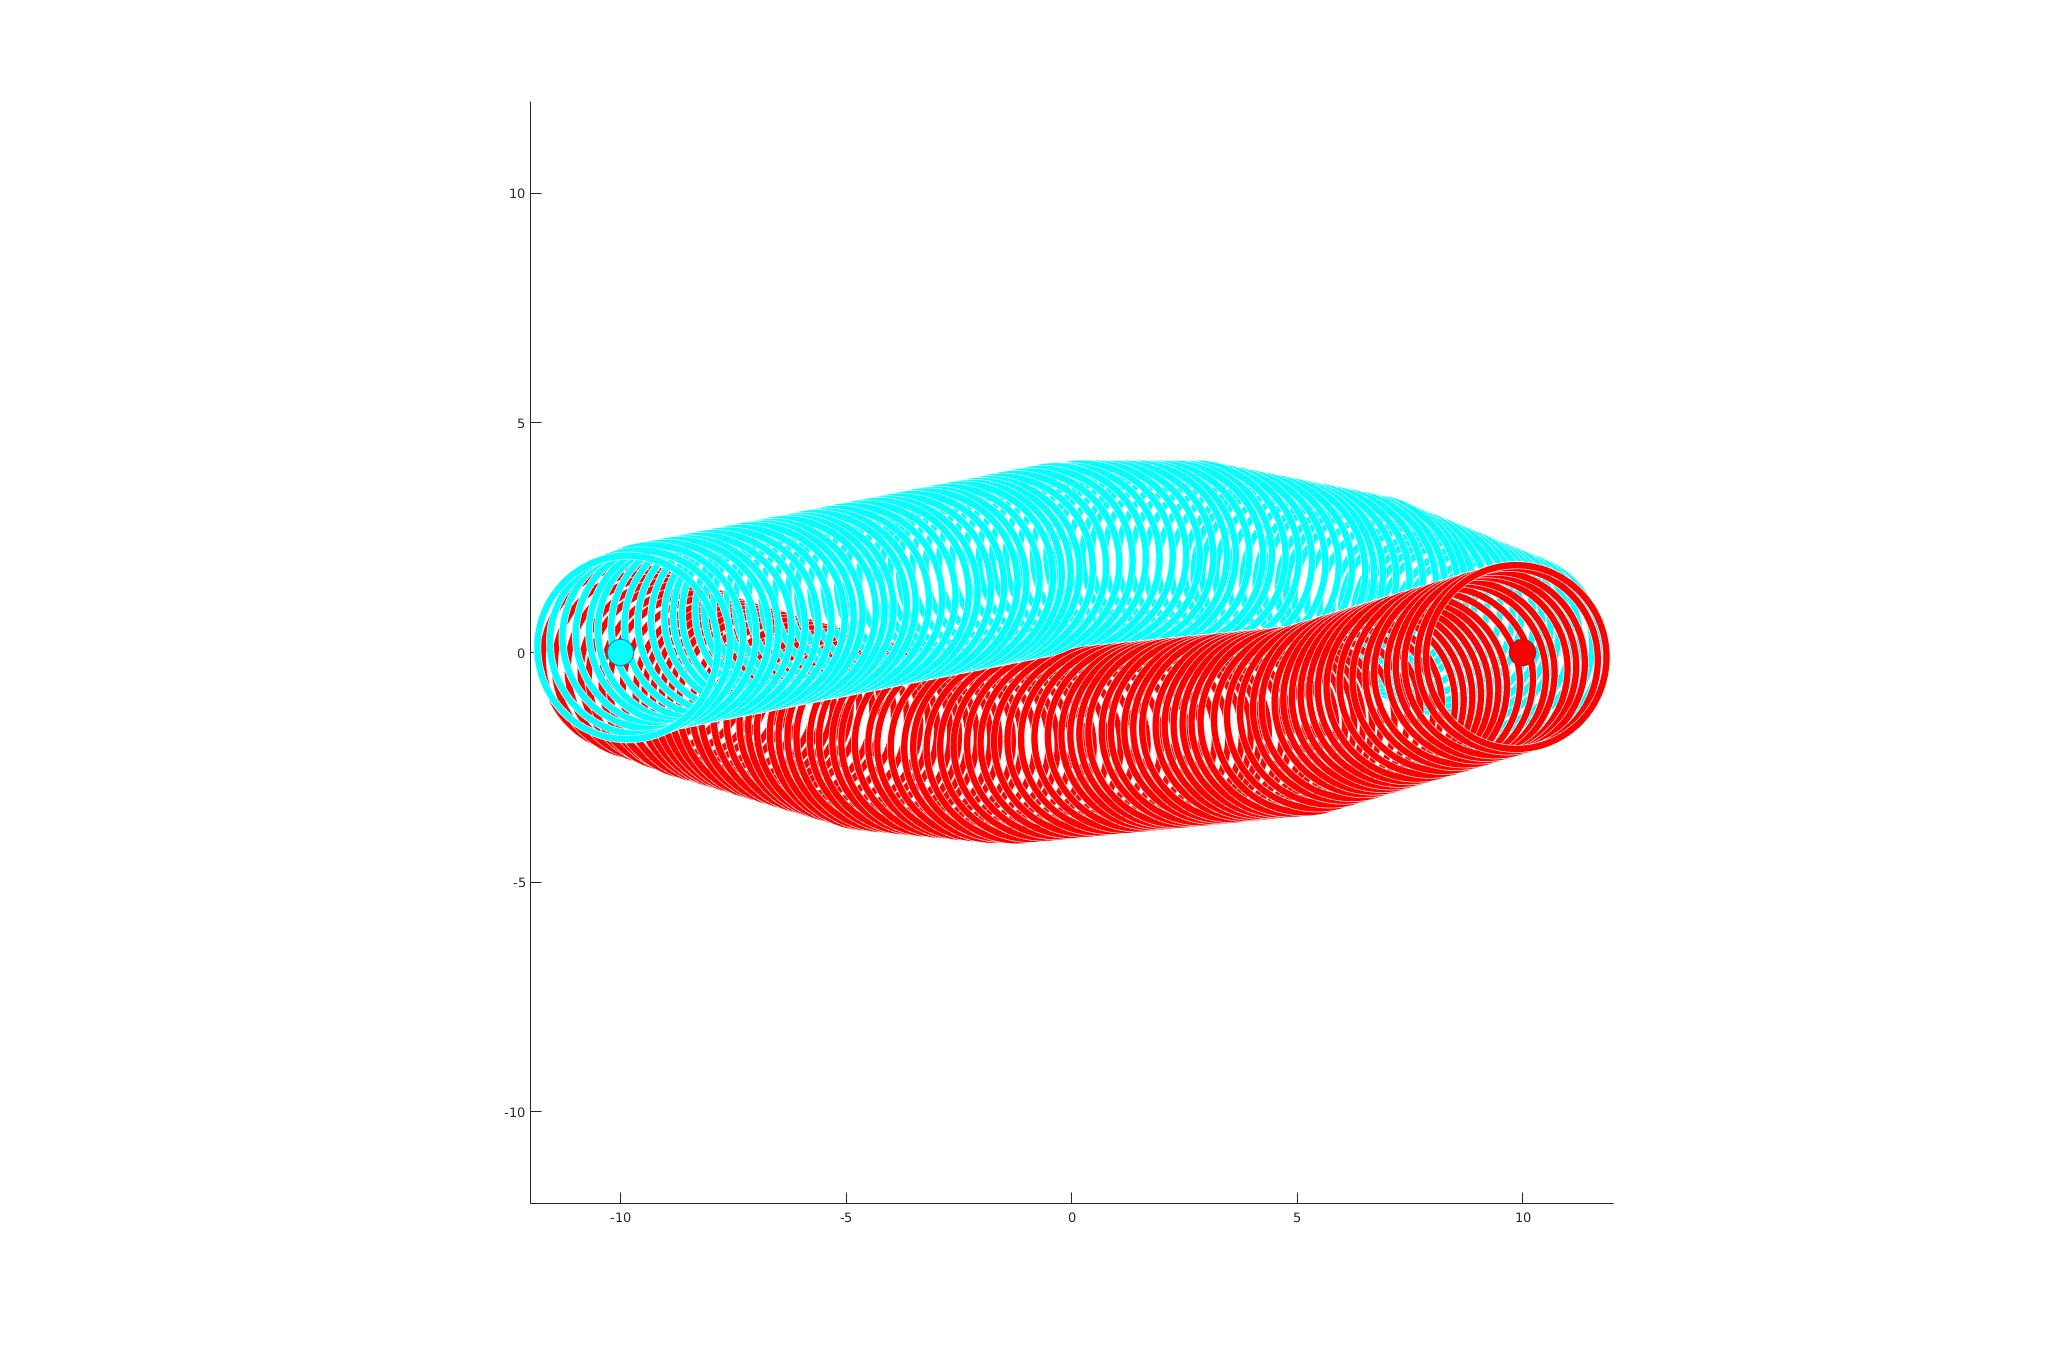
\includegraphics[width=.48\columnwidth]{Due}} \quad
\subfloat[Sei agenti di raggio 1]
{\label{fig:}
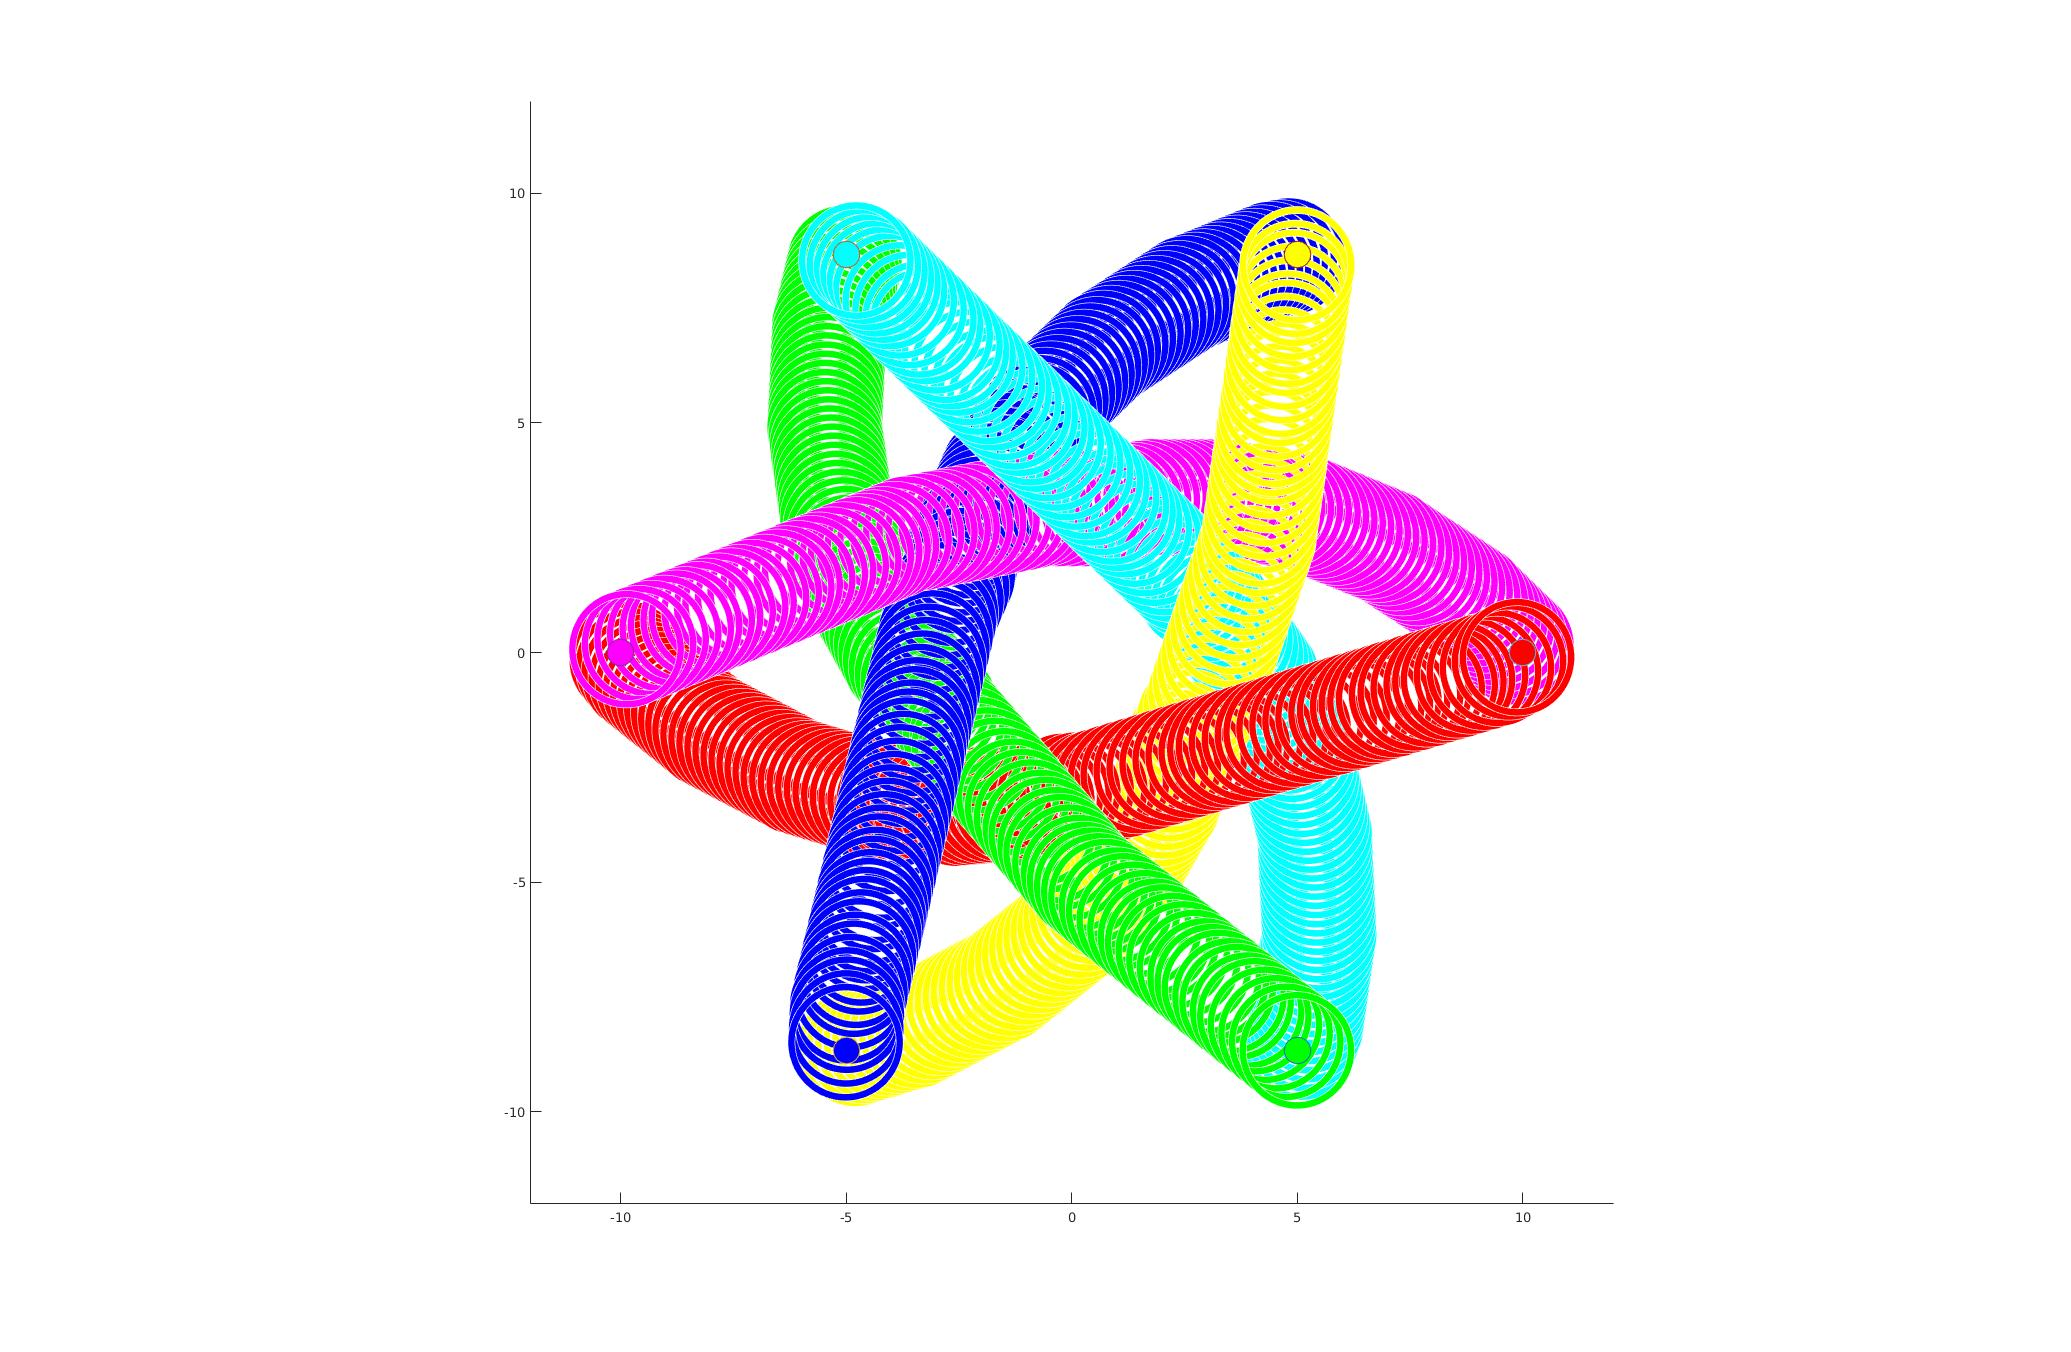
\includegraphics[width=.48\columnwidth]{sei}} \\
\subfloat[Dodici agenti di raggio random]
{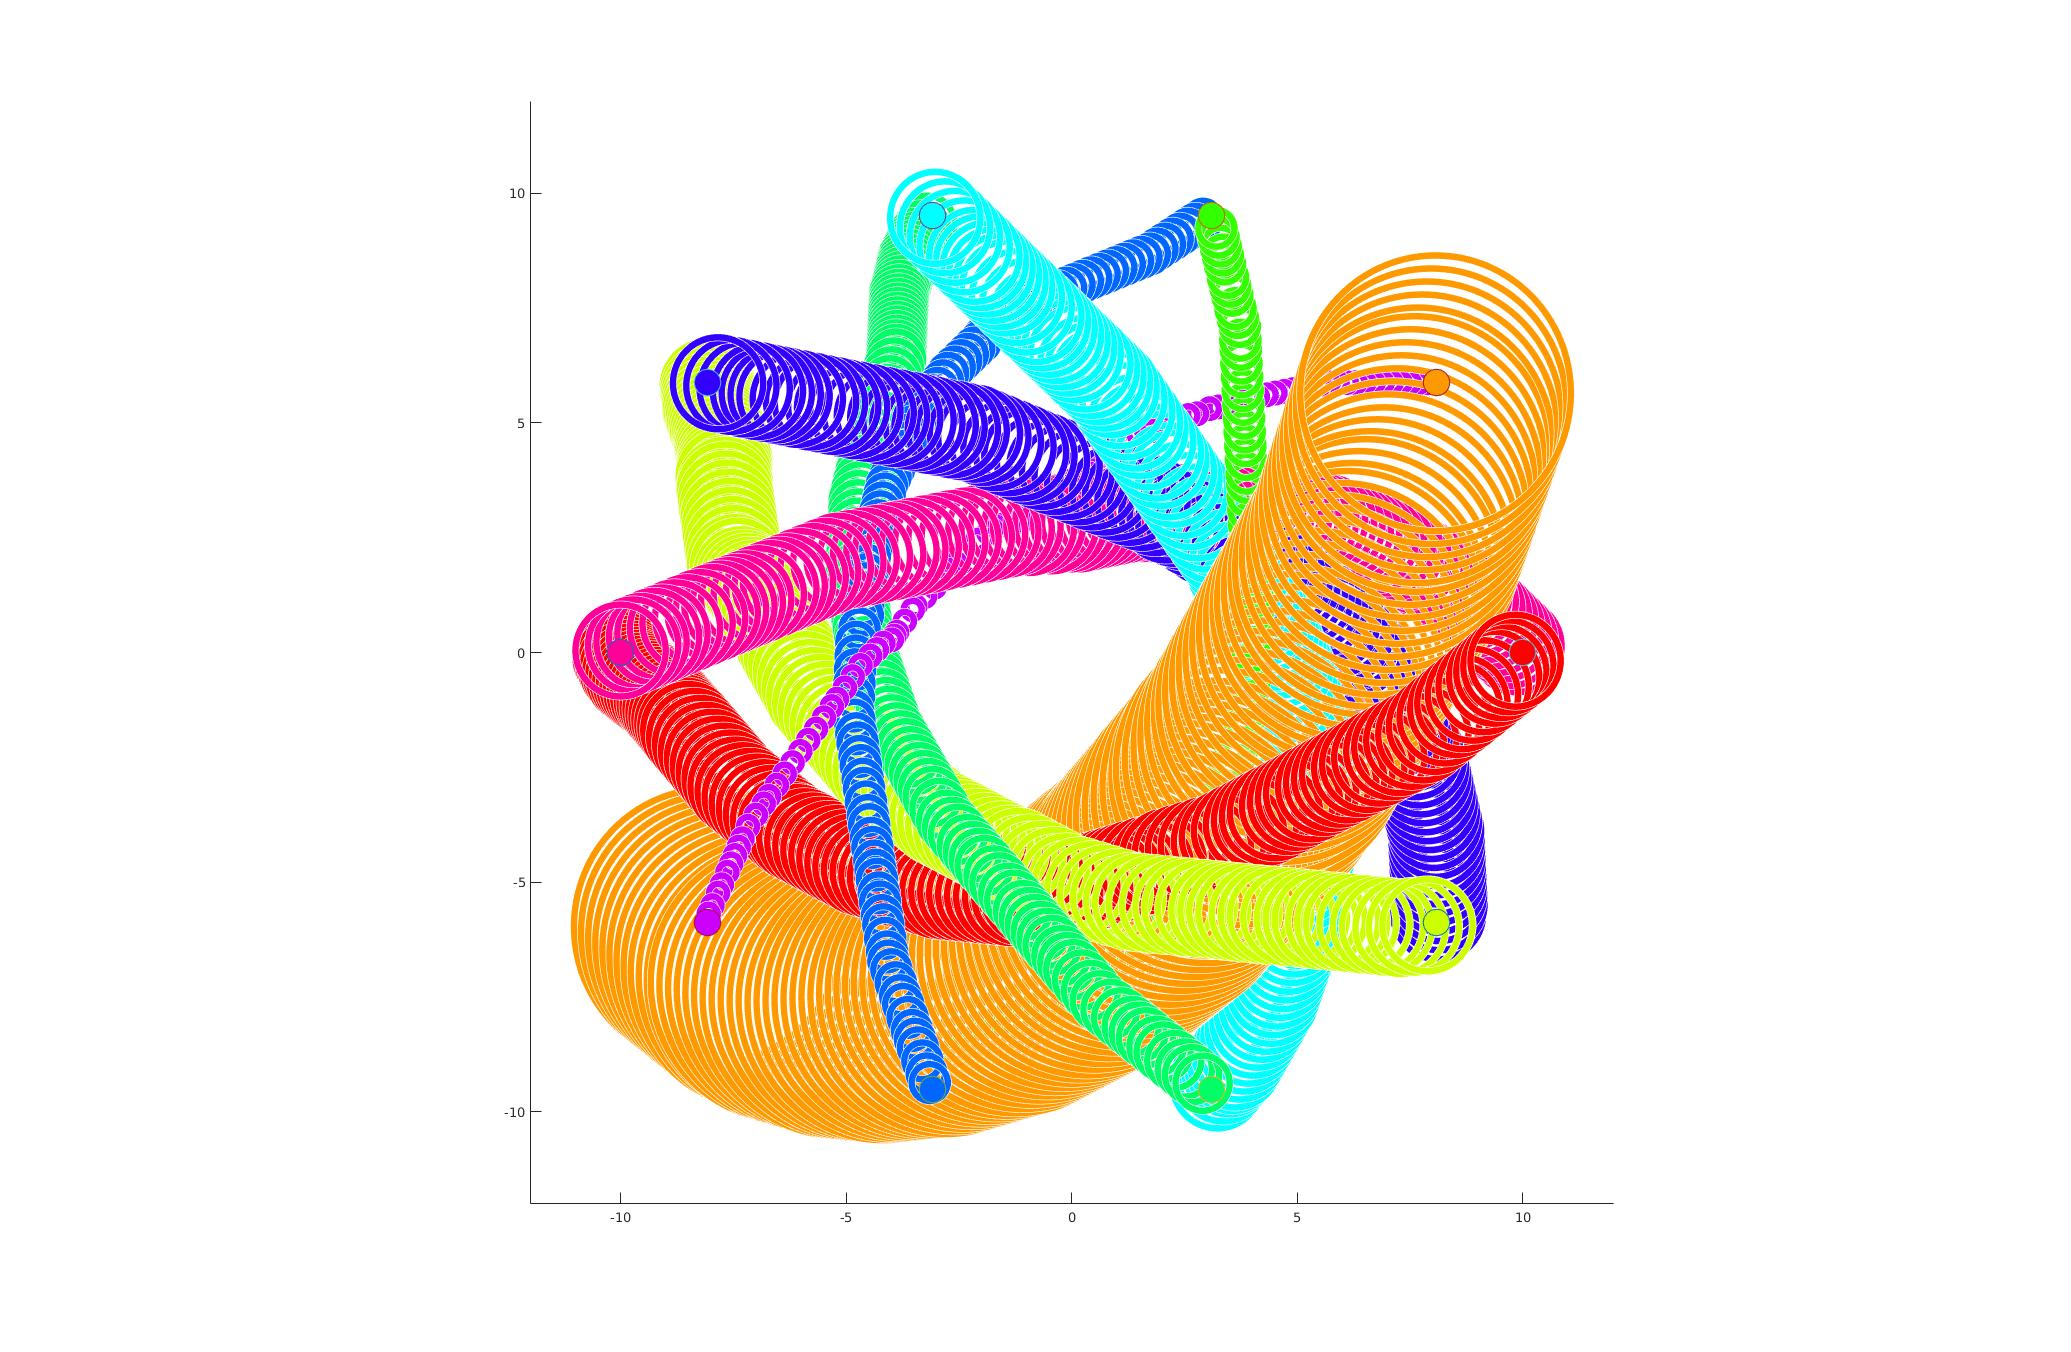
\includegraphics[width=.48\columnwidth]{random}} \quad
\subfloat[Tre agenti di raggio 1]
{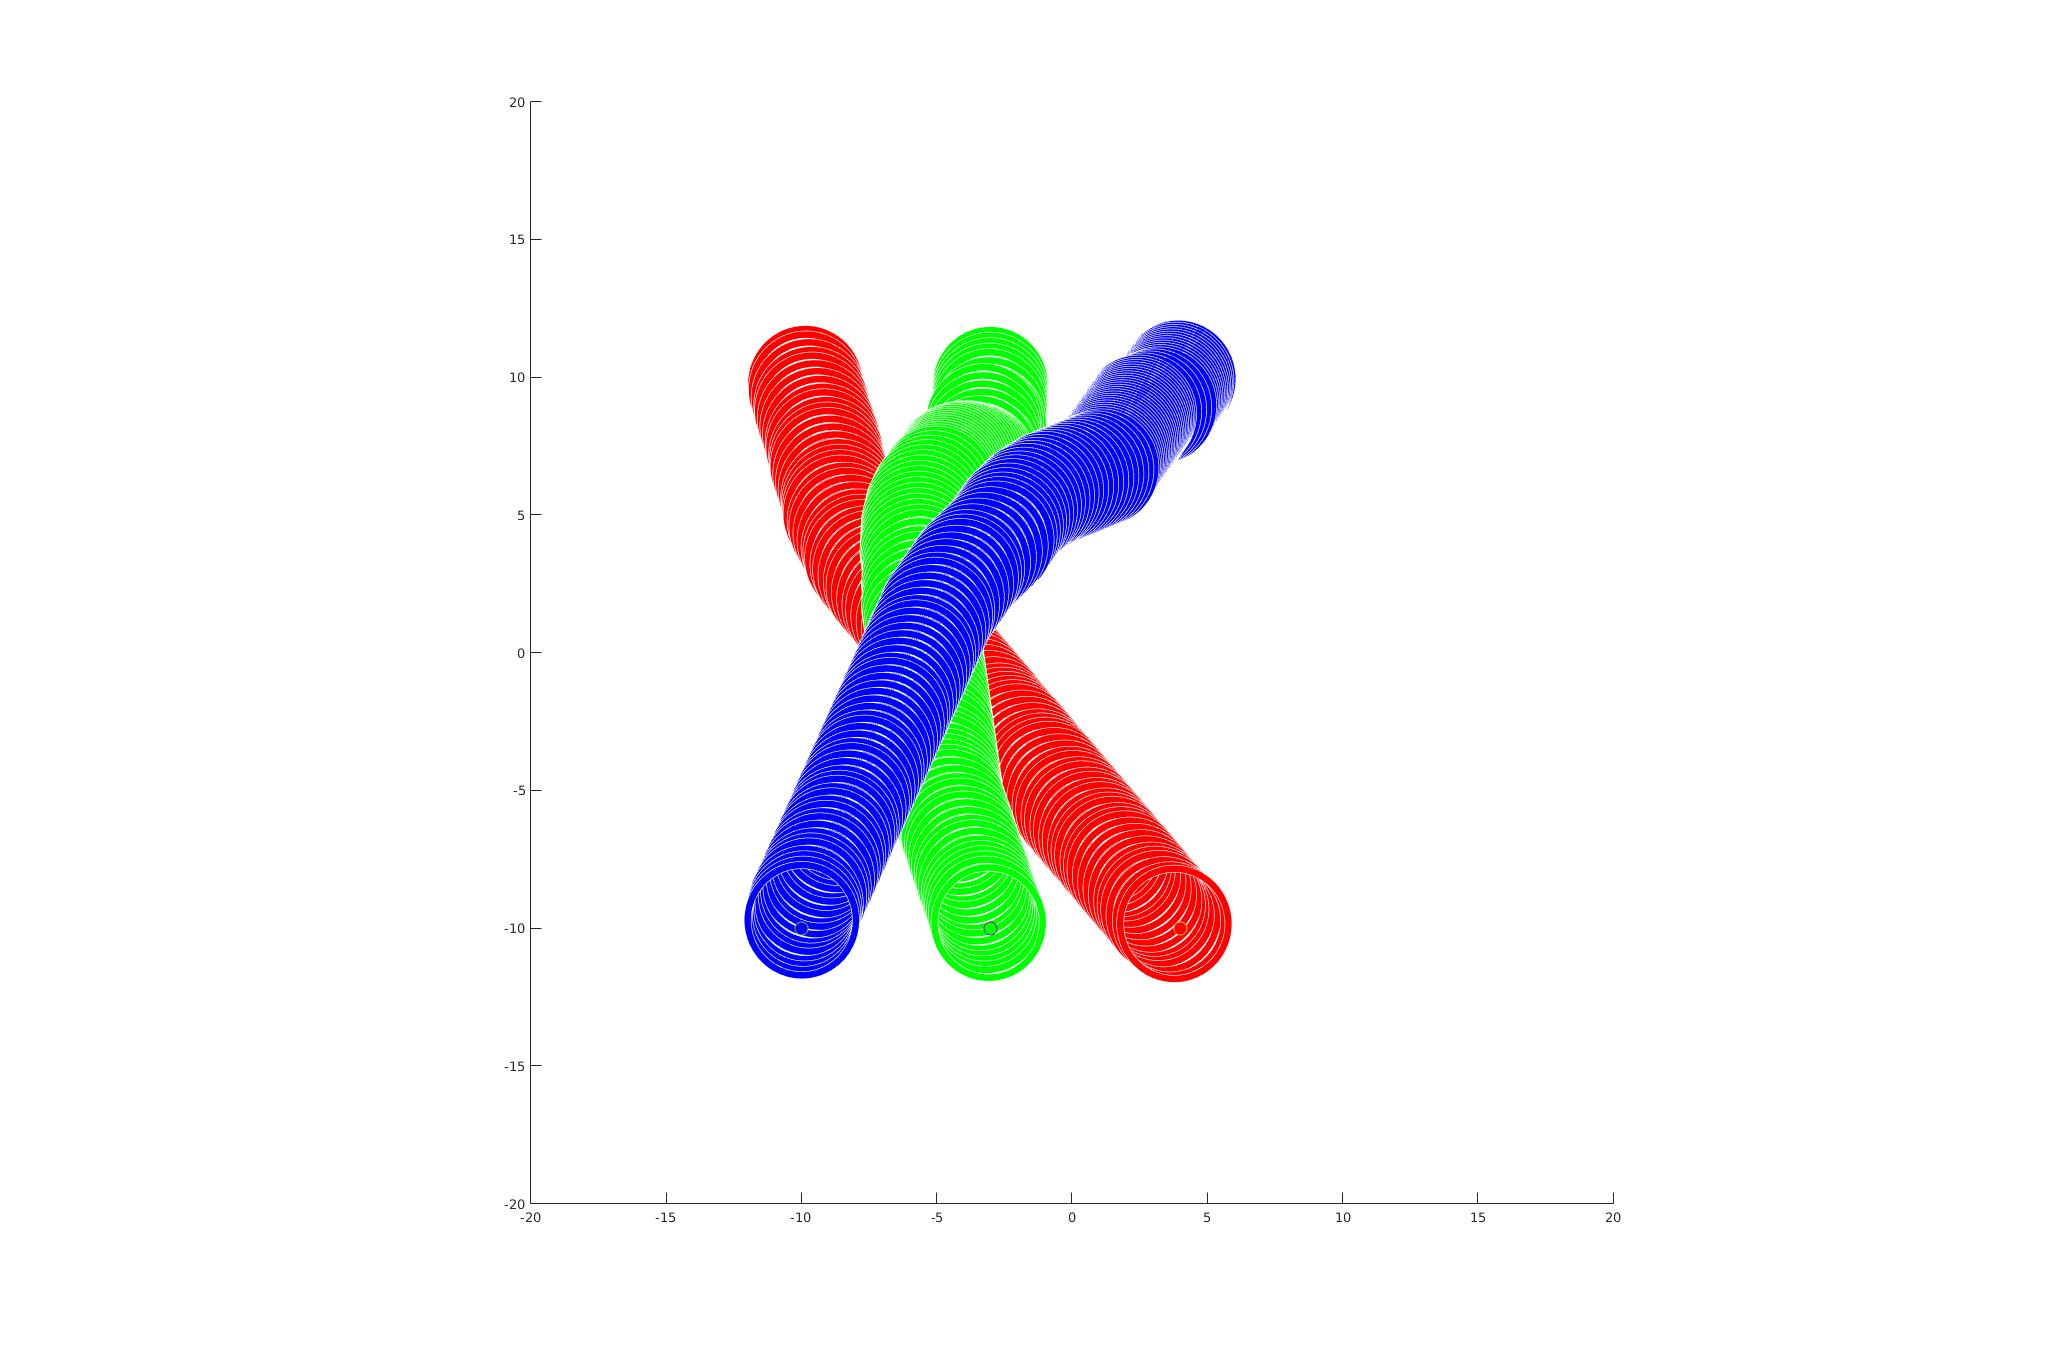
\includegraphics[width=.48\columnwidth]{X3}}
\caption[a,b,c,d dei risulati della simulazione]{Stampa delle traiettorie della simulazione}
\label{fig:}
\end{figure}
\newpage
\subsection{Risulati con $\tau$}
Mi sono posto lo stesso problema con l'aggiunta di utilizzare un cono troncato utilizzato nelle ORCA, questi sono i risultati:
\begin{itemize}
\item le traiettorie sono pi\'u rettilinee.
\item gli agenti nella parte centrale sono pi\'u vicini rispetto a non utilizzarlo.
\item con l'aumento di densit\'a della popolazione della scena \'e meglio utilizzare un $\tau$ maggiore di 2.
\end{itemize}



\begin{figure}
\centering
\subfloat[Due agenti di raggio 2]
{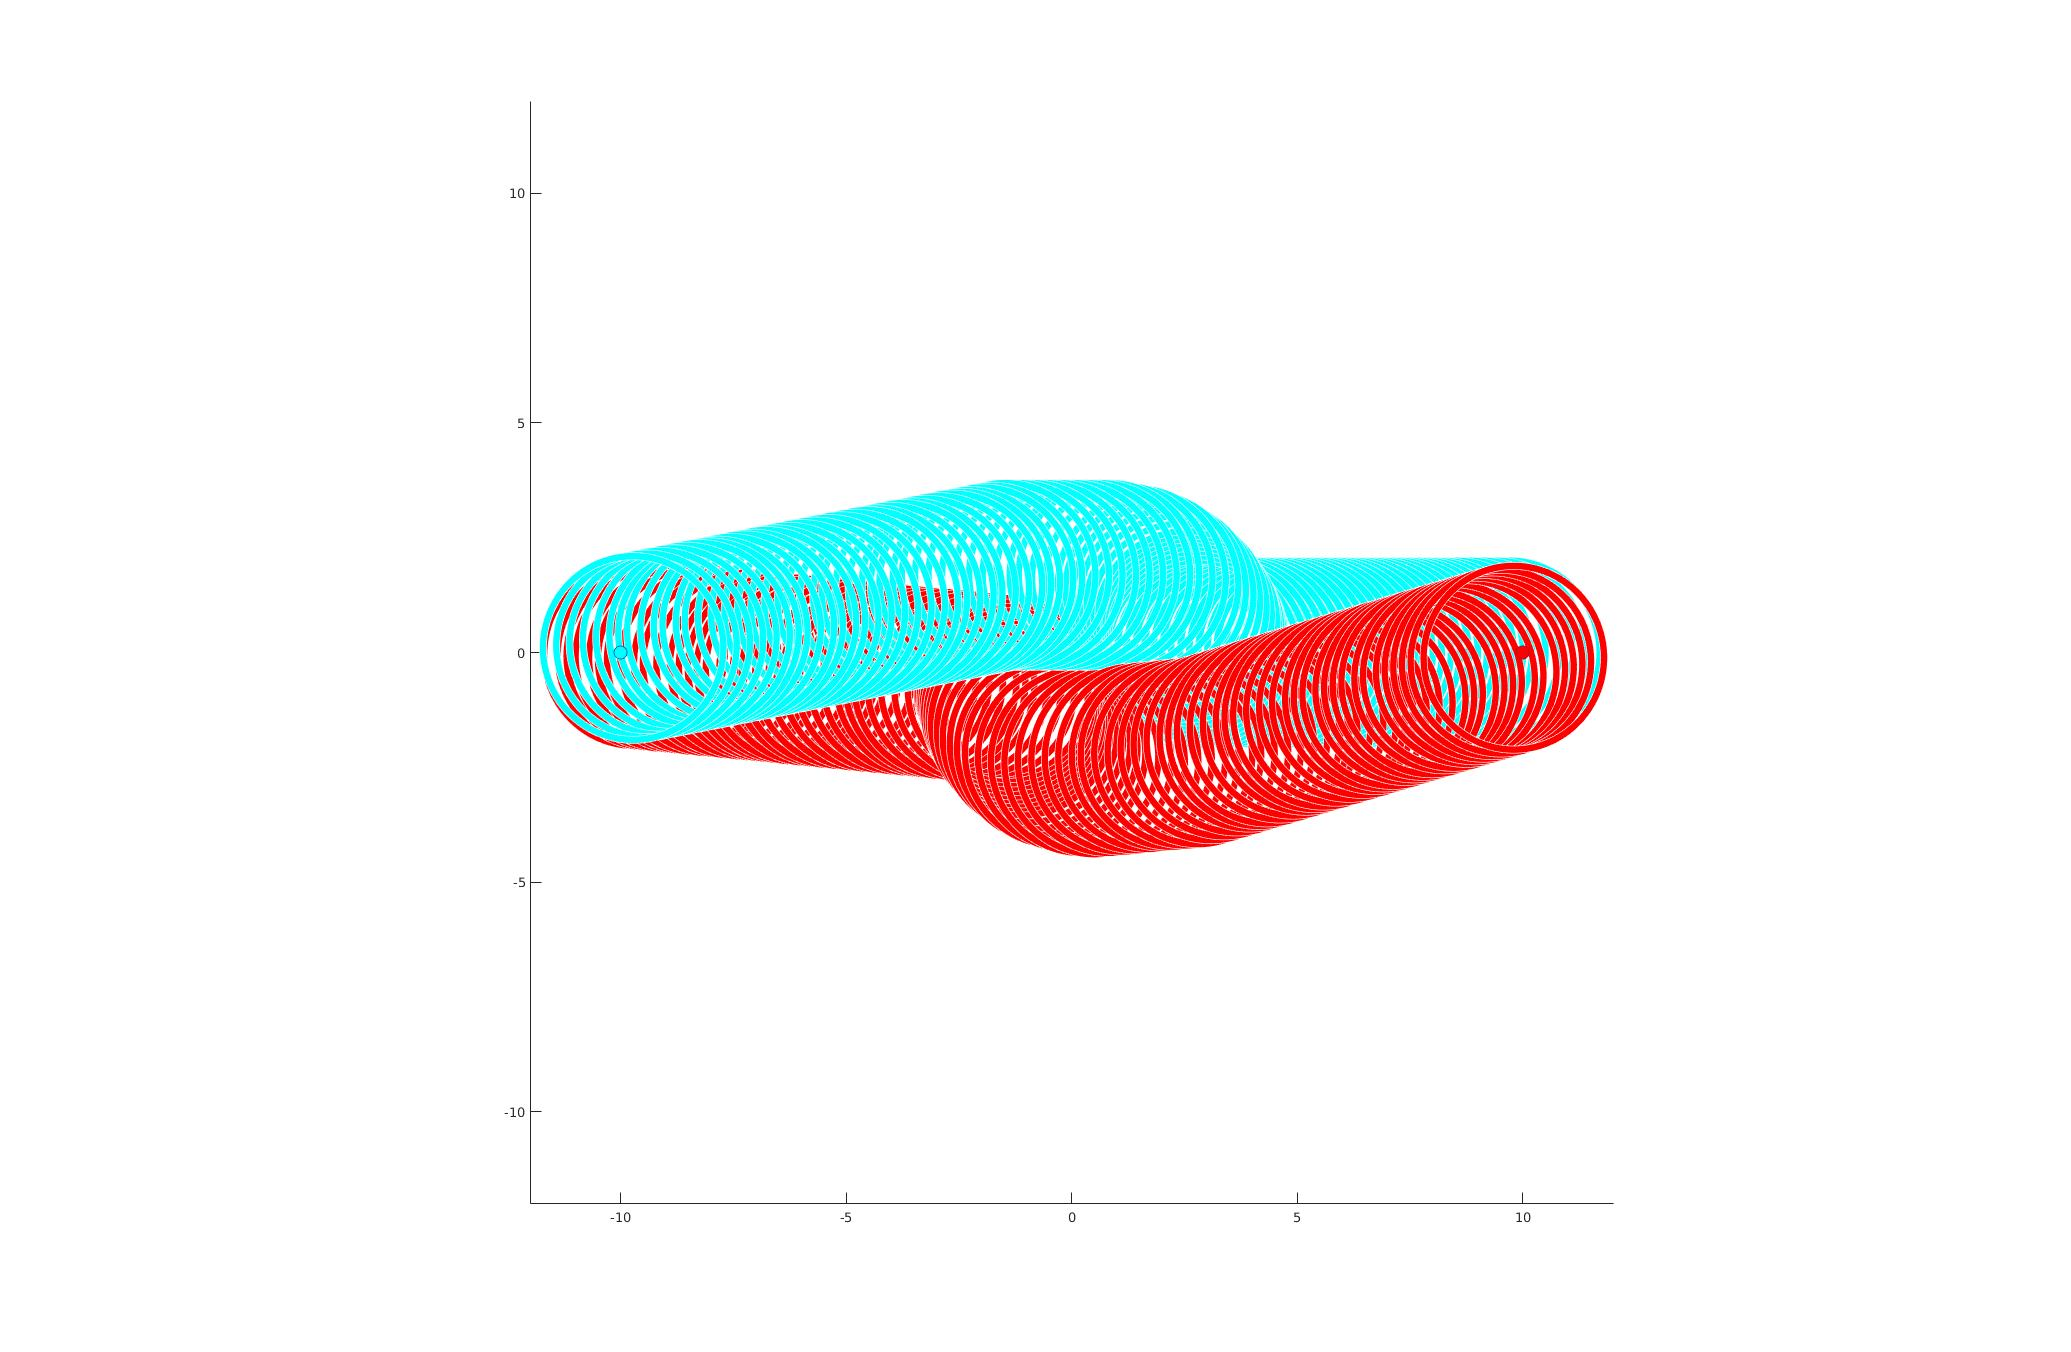
\includegraphics[width=.48\columnwidth]{2tau}} \quad
\subfloat[Sei agenti di raggio 1]
{\label{fig:}
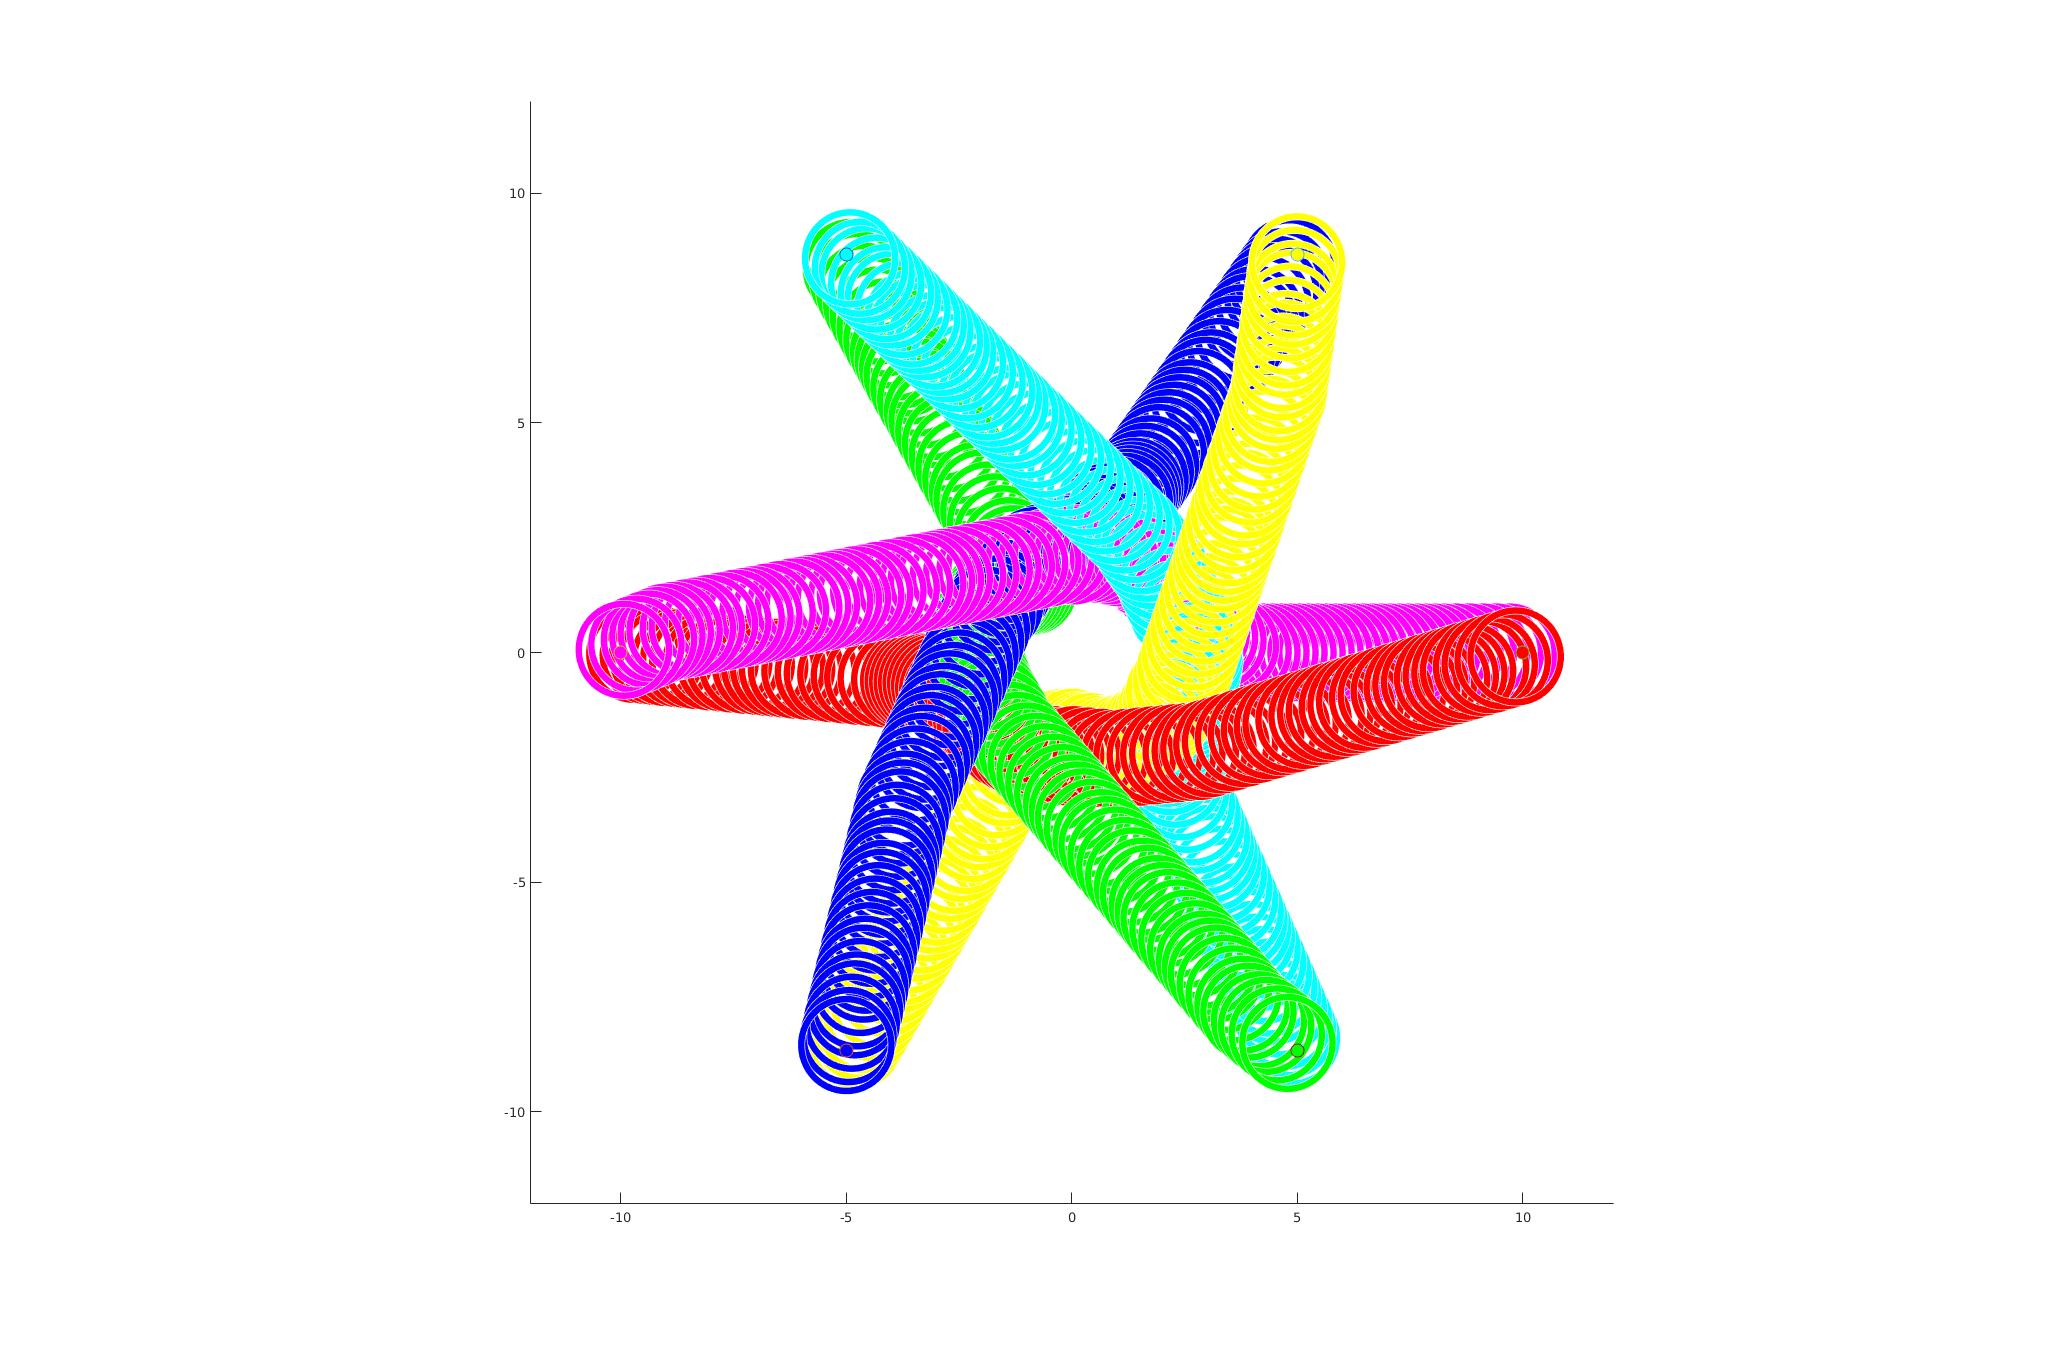
\includegraphics[width=.48\columnwidth]{6tau}} \\

\subfloat[Tre agenti di raggio 1]
{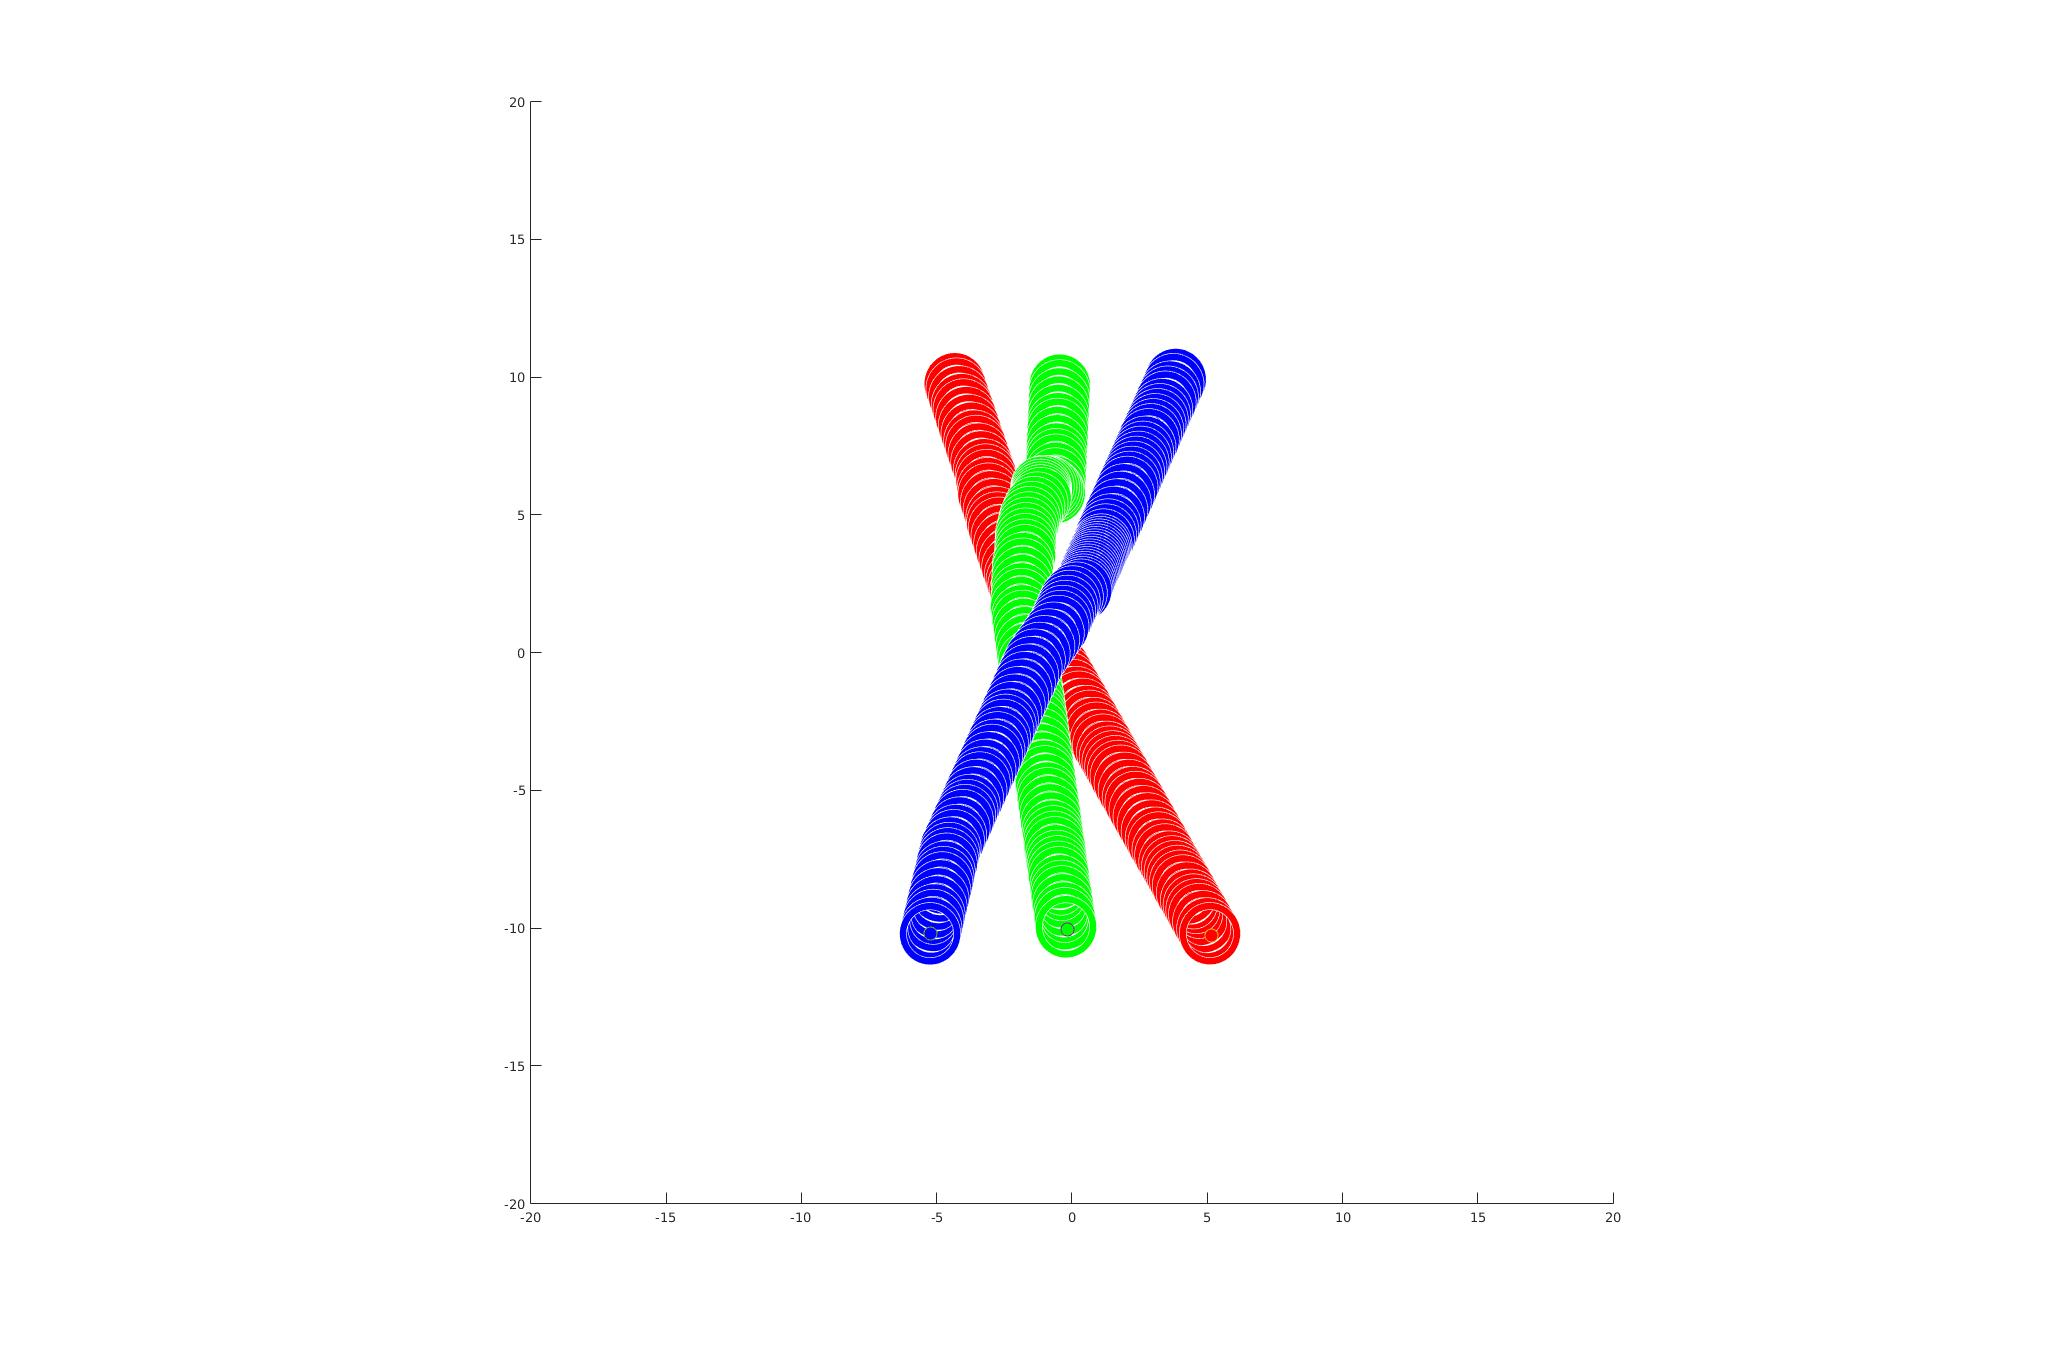
\includegraphics[width=.48\columnwidth]{3Xtau}}
\caption[a,b,c,d dei risulati della simulazione con $\tau$]{Stampa delle traiettorie della simulazione con $\tau$}
\label{fig:}
\end{figure}


